
We describe  \sys's architecture and basic operation in Section~\ref{ssec:overview}.
We then discuss in-memory compaction policies  in  Section~\ref{ssec:policies}
and implementation details and thread synchronization in Section~\ref{ssec:impl-details}.
\inred{ 
Section~\ref{ssec:offheap} discusses off-heap allocation of  the flat memory segments.
}

\subsection{Overview} \label{ssec:overview}

\begin{figure}[tbh]
\center
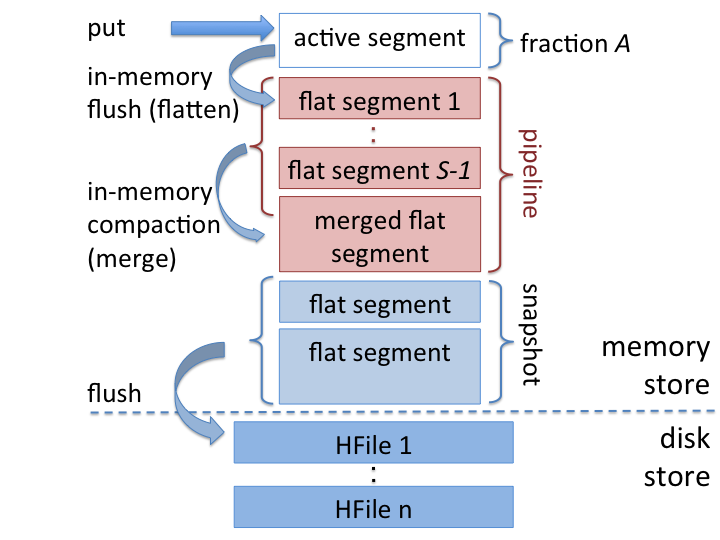
\includegraphics[width=\columnwidth]{accordion-arch} 
\caption{\sys's compacting memory store architecture adds a pipeline of flat segments between the active segment and the snapshot. 
The memory store includes a small dynamic active segment 
and a pipeline of flat segments. A disk flush creates a snapshot of the pipeline for writing to disk.}
\label{fig:accordion}
\end{figure}

\sys\ introduces a \emph{compacting} memory store to the LSM tree design framework. In contrast to the traditional memory store, 
which maintains RAM-resident data in a single monolithic data structure, \sys\ manages data as a \emph{pipeline} of 
\emph{segments} ordered by creation time. \inred{Each segment is an index over a collection of data cells.}
At all times, the most recent segment, called \emph{active}, is mutable;
it absorbs put operations. The rest of the segments are immutable.  
%
Get and scan operations retrieve data from all  segments,  similarly to a traditional LSM tree read from multiple files. 
  
Figure~\ref{fig:accordion} illustrates the \sys\ architecture. It is parameterized by two values:
\begin{itemize}
\item  $A$ --  fraction of the memory store allocated to the active segment; and 
\item $S$ --  upper bound on the number of immutable segments in the pipeline. 
\end{itemize}

\noindent
As our experiments show (Section~\ref{sec:eval}), the most effective parameter values are quite small, 
e.g., $0.02 \leq A \leq 0.05$, and $1 \leq S \leq 5$.

Once the active segment grows to its size bound (a fraction $A$ of the memory store's size bound), an \emph{in-memory flush} is invoked.
The in-memory flush makes the active segment immutable and creates a new active segment to replace it. 

The replaced active segment is then \emph{flattened} and added to the pipeline.
This involves replacing the dynamic segment index (e.g., skiplist) by a compact ordered array, 
which is suitable for immutable data and supports fast lookup via binary search. 
\inred{The indexed data cells are unaffected by the index's flattening.}
Flattening reduces the MemStore's memory footprint, which delays  disk flushes, positively affecting both read latency  (by increasing the MemStore's hit rate) and write volume.
\inred{
  An additional advantage of the flat layout  is that in managed environments, 
 the index can be allocated in off-heap (unmanaged) memory, which can improve performance predictability 
 through reduced garbage collection jitter~\cite{alibabahbase}; this approach is  discussed in Section~\ref{ssec:offheap} below.
 }


In case there is available space in the pipeline (the number of pipeline segments is smaller than $S$), 
the flattened segment is simply added to the pipeline and the memory flush takes no further actions.  
Once the number of immutable segments exceeds $S$, \emph{in-memory compaction} occurs. 
At a minimum, compaction replaces the indices of multiple segments by a single index covering data that was 
indexed by all original segments. This is a lightweight process that does not eliminate redundant data versions.

Optionally, it can further perform \emph{redundant data elimination} by
creating a flat index with no redundancies and disposing redundant data cells. 
\inred{ 
In case the memory store manages its cell data storage internally (off-heap), the surviving cells are relocated
to a new contiguous buffer. Otherwise, the redundant cells are simply de-referenced, allowing the garbage-collector to reclaim them.    
}
%
The choice whether to eliminate redundant data or not is guided by the policies described in Section~\ref{ssec:policies} below.

Flushes to disk work the same way as in a standard LSM tree: A disk flush first shifts all pipeline segments to the snapshot, which is not part of the pipeline, while the pipeline is emptied so that
it may absorb new flat segments. 
A background flush process merges all snapshot segments while eliminating  redundancies, and streams the result to a new file. 
After the file is written, the snapshot segments are freed. 

In case the disk flush process empties the pipeline while an in-memory compaction  is attempting to merge some segments, the latter aborts.  This behavior is valid since in-memory compactions are an optimization.

\subsection{Compaction Policies} \label{ssec:policies}

Redundant data elimination induces a tradeoff. On the one hand,
merging only search indices without removing redundancies is a lighter-weight process.  
Moreover, this approach is friendly to the managed memory system because the entire segment is freed at once, whereas 
removing (redundant) cells from existing segments burdens the memory management system (in particular, the garbage collector) by
constantly releasing small objects. On the other hand, by forgoing redundant data elimination we continue to 
consume memory for overwritten data; this is significant in production-like heavy-tailed distributions where some keys are frequently overwritten.
Removing these redundancies further delays disk flushes, which both improves read latency  (thanks to more 
queries being satisfied from memory) and reduces the write volume.

Our HBase 2.0 implementation includes the two extreme memory compaction policies:
\begin{description}
\item[\basic] (low-overhead) never performs redundant data elimination. Rather, 
once a segment becomes immutable, flattens its index, and once the pipeline size exceeds $S$, merges all segment indices into one.   
\item[\eager] (high-overhead, high-reward under self-similar workloads) immediately merges a segment that becomes immutable 
with the current  (single) pipeline segment, while eliminating redundant data.
%Once a segment becomes immutable, merge its index and data with the current (single) pipeline segment.
% In addition to \basic\/ mechanisms, eliminate data redundancies across pipeline segments.
\end{description}

Our experiments (reported in the next section) show that the \eager\ policy is typically too aggressive, in particular when $A$ is small,
and the benefits from reducing the memory footprint are offset by the increased management (and in particular, garbage collection) overhead.
We therefore present in this paper a third policy:
\begin{description}
\item[\adp] (the best of all worlds)\footnote{\small{Not committed to production code yet.}}. A heuristic that chooses 
whether to eliminate redundant data  (as in \eager) or not (as in \basic) based on the level of redundancy in the data 
and the perceived cost-effectiveness of compaction. \adp\ works at the level of a single LSM store, i.e., triggers 
redundancy elimination only for those stores where positive impact is expected. 
\end{description}

\adp\ uses two parameters to determine whether to perform data redundancy elimination:
\begin{enumerate}
\item
%The first is 
A throttling parameter $t$  grows with the amount of data that can benefit from redundancy elimination. 
Initially, $t=0.5$; it then grows exponentially by $2\%$ with the number of in-memory flushes, and is reset back to 
the default value (namely $0.5$) upon disk flush. Thus, $t$ is bigger when there is more data in the MemStore.
\item
The \emph{uniqueness} parameter, $u$, estimates the ratio of unique keys in the memory store based on the 
fraction of unique keys encountered during the previous merge of segment indices. 
\end{enumerate}

Note that the accuracy of $u$ at a given point in time depends on the number of merges that occurred since the last disk flush
or data-merge.
Initially, $u$ is zero, and so the first in-memory compaction does not employ data-merge.
Then, the estimate is based on the $S$ merged components, which at the time for the second in-memory compaction
is roughly one half of the relevant data, since the pipeline holds $S-1$ unmerged components. 
Over time, $u$ becomes more accurate while $t$ grows. 

\adp\/ triggers redundancy elimination with probability $t$ if the fraction of redundant keys $1-u$ exceeds a parameter 
threshold $R$. The rationale for doing so is that prediction based on $u$ becomes more accurate with time, whence 
compactions become more important because the component is bigger and more space can be saved.


\remove{
\begin{description}
\item[\emph{Unique ratio}] $u$ -- an estimate of the fraction of unique keys out of the total number of items in the segment. 
This value is estimated by counting duplicates encountered during merge, which does not induce extra overhead since
merged items are compared in any case. The \emph{unique\_ratio}  is an under-estimate of the actual redundancy because it does not 
take into consideration duplicates that were already present during flattening. Nevertheless, since the active component
is typically quite small, the error due to the under-estimate is significant only when the component is still small 
(has not undergone many merges), and compaction is therefore less important.
\item[\emph{success\_probability}] -- an estimate of the probability of a compaction yielding the expected benefits based on recent history.
Here, we define an expected space reduction threshold below which compaction is not cost-effective. 
We initialize the \emph{success\_probability} to some default value (e.g., $0.5$). 
Then, if compaction yields the expected benefit (i.e., frees up more space than the threshold) we increase the \emph{success\_probability},
and otherwise decrease it. The \emph{success\_probability} is reset to its default value upon flushes. 
The rationale for using \emph{success\_probability} is that its prediction becomes more accurate with time, whence 
compactions become more important because the component is bigger and more space can be saved.
\end{description}
}

\subsection{Concurrency} \label{ssec:impl-details}

A compacting memstore is comprised of an active segment and a double-ended queue (pipeline) of inactive segments. 
The pipeline is accessed by read APIs (get and scan), as well as by background disk flushes and in-memory compactions. 
The latter two modify the pipeline by adding/removing/replacing segments. These modifications happen infrequently. 

The pipeline's readers and writers coordinate through lightweight copy-on-write, as follows. The pipeline object is versioned. 
Each modification promotes the version number, and atomically swaps the global reference to the new version clone. Note
that cloning is inexpensive -- only the segment references are copied since the segments themselves are immutable. 

The reads access the segments lock-free, through the version obtained at the beginning of the operation. If a disk flush
is scheduled in the middle of a read, a segment may migrate from the pipeline to the pre-flush snapshot buffer. The correctness of
reads  is guaranteed by scanning the pipeline clone first. This way, a segment may be encountered twice but no data is 
lost. The scan algorithm filters out the duplicates. 

In-memory compaction is a read-modify-write operation, which swaps one or more segments in the pipeline 
with a new segment built from their data. This operation's atomicity is guaranteed by a compare-and-swap (CAS) operation
that flips the pipeline version only if the latter did not change since the compaction started.  For example, in-memory
compaction fails if a disk flush concurrently removes some segments from the pipeline.
% (Section~\ref{ssec:overview}). 

\inred{
\subsection{Off-Heap  Allocation} \label{ssec:offheap}
Prior to \sys, HBase allocated its MemStore on-heap, using a standard Java skiplist for the active buffer and an
array for the snapshot. \sys\ continues to use the same data structures -- skiplist for the active segment and arrays for the flat ones. 
Each skiplist node or array entry holds a reference to a \emph{cell} object, which holds a reference to a buffer holding a key-value pair,
as illustrated in Figure~\ref{fig:on-heap}. 
The cell object is used for internal HBase scan APIs, and can reference data in two different formats: either a standard Java object
called \emph{pojo} -- Pure Old Java Object -- or an address in a bulk-allocated array called \emph{mslab} -- Memory Slab. 
HBase mslabs may be allocated off-heap. 

\begin{figure}[tbh]
\center
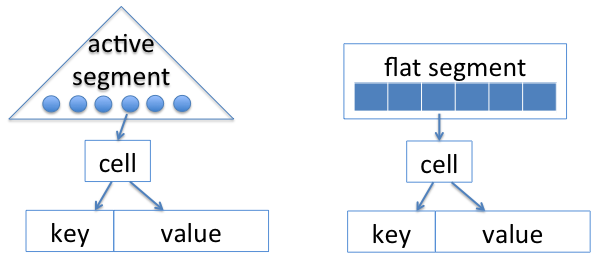
\includegraphics[width=0.9\columnwidth]{on-heap} 
\caption{Standard on-heap allocation with cell objects.}
\label{fig:on-heap}
\end{figure}
\begin{figure}[tbh]
\center
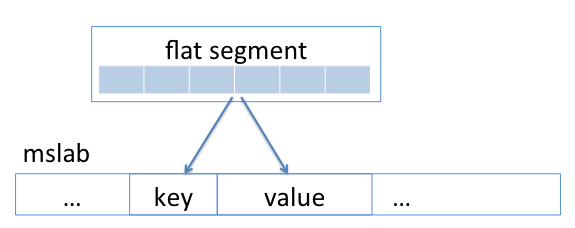
\includegraphics[width=0.75\columnwidth]{off-heap} 
\caption{Off-heap allocated flat segment referencing data that resides in mslabs.}
\label{fig:off-heap}
\end{figure}


\sys's off-heap version takes this approach one step further, and allocates the flat segments off-heap as well. It therefore forgoes the intermediate cell
objects, and has the  array entries in the off-heap flat segments point directly to the the off-heap mslabs as illustrated in Figure~\ref{fig:off-heap}.  
Removing the cell objects yields
a substantial space reduction, especially when data items are small. However, it necessitates recreating temporary
cell objects to support HBase's internal scan APIs. Nevertheless, such temporary objects consume  a small amount of space on-demand, 
and these objects are  deallocated rapidly, making them easier for the GC process to handle.

}




